% ============================================================
%  Dal-i — Presentació Sistemes Multimedia · UAB · Juny 2026
%  Compilar amb:  latexmk pres.tex
% ============================================================
\documentclass[12pt, aspectratio=169]{beamer}

% ── Tema ────────────────────────────────────────────────────
\usetheme{metropolis}
\setbeamertemplate{navigation symbols}{}
\metroset{progressbar=frametitle}

% ── Idioma i fonts (LuaLaTeX) ───────────────────────────────
\usepackage{fontspec}
\usepackage[catalan]{babel}
\usepackage{microtype}

% ── Icones vectorials (FontAwesome 5, inclòs a TeXLive) ─────
\usepackage{fontawesome5}

% ── Gràfics i colors ────────────────────────────────────────
\usepackage{graphicx}
\usepackage{xcolor}
\usepackage{booktabs}
\usepackage{tikz}
\usetikzlibrary{arrows.meta, positioning, calc}

% ── Color accent personalitzat ──────────────────────────────
\definecolor{dalblue}{HTML}{1A73E8}
\setbeamercolor{alerted text}{fg=dalblue}
\setbeamercolor{progress bar}{fg=dalblue}
\setbeamercolor{frametitle}{bg=black!85, fg=white}

% ── Macro per a placeholders d'imatge ───────────────────────
\newcommand{\imgplaceholder}[2][5cm]{%
  \fbox{\parbox[c][#1][c]{0.9\linewidth}{%
    \centering\small\ttfamily\color{gray} #2}}%
}

% ── Metadades ────────────────────────────────────────────────
\title{\textbf{Dal-i}}
\subtitle{Sistema Robòtic de Dibuix Col·laboratiu}
\author{Grup G4-6}
\institute{Sistemes Multimèdia · UAB}
\date{5 de juny de 2026}

% ============================================================
\begin{document}

% ── Diapositiva 1: Portada ───────────────────────────────────
\begin{frame}[plain, noframenumbering]
  % Capçalera fosca estil metropolis (més estreta per donar espai al logo)
  \begin{beamercolorbox}[wd=\paperwidth, ht=1.8cm, dp=0.3cm,
      leftskip=0.9cm, rightskip=0.9cm]{frametitle}
    \vspace{0.25cm}
    {\usebeamerfont{title}\color{white}\inserttitle}\par
    {\usebeamerfont{subtitle}\color{white!75!black}\insertsubtitle}
  \end{beamercolorbox}

  \vspace{0.15cm}

  \begin{columns}[c]
    % ── Esquerra: info del grup + taula ───────────────────
    \begin{column}{0.50\textwidth}
      \hspace{0.9cm}%
      \begin{minipage}{0.88\linewidth}
        {\usebeamerfont{author}\insertauthor}\par
        \smallskip
        {\small\color{gray}\insertinstitute}\par
        \smallskip
        {\small\color{gray}\insertdate}\par
        \vspace{0.4cm}
        \small
        \begin{tabular}{@{}l r@{}}
          \toprule
          \textbf{Nom i Cognoms}    & \textbf{NIU} \\
          \midrule
          David Madueño Noguer      & 1526933 \\[2pt]
          Moisés Sánchez Pin        & 1603611 \\[2pt]
          Xavier Cañada Escalona    & 1708948 \\[2pt]
          Lorenzo Payaro Robles     & 1731940 \\
          \bottomrule
        \end{tabular}
      \end{minipage}
    \end{column}

    % ── Dreta: logo gran ──────────────────────────────────
    \begin{column}{0.46\textwidth}
      \centering
      
\includegraphics[width=0.82\linewidth]{images/logo.jpeg}
    \end{column}
  \end{columns}
\end{frame}


% ── Diapositiva 2a: Idea i Aplicació ────────────────────────
\begin{frame}{Idea i Aplicació}
  \begin{columns}[c]

    \begin{column}{0.55\textwidth}
      \vspace{0.5cm}

      \begin{tikzpicture}[
        node distance=0.5cm,
        box/.style={draw, rounded corners, fill=dalblue!10,
                    inner sep=4pt, font=\small},
        arr/.style={-{Stealth}, thick, color=dalblue}
      ]
        \node[box] (img)  {Imatge + Estil};
        \node[box] (edge) [right=of img]  {Contorns};
        \node[box] (bot)  [right=of edge] {Robot};
        \draw[arr] (img)  -- (edge);
        \draw[arr] (edge) -- (bot);
      \end{tikzpicture}

      \medskip
      \begin{itemize}
        \item Entrada per \alert{veu}, \alert{text} o selecció ràpida
        \item Mode Avançat: \alert{Gemini} genera transformació visual
        \item \alert{10 idiomes}: traducció automàtica interna
      \end{itemize}
    \end{column}

    \begin{column}{0.42\textwidth}
      \centering
      
\includegraphics[width=0.85\linewidth]{images/logo.jpeg}
    \end{column}

  \end{columns}
\end{frame}

% ── Diapositiva 2b: Captura de l'aplicació ───────────────────
\begin{frame}{L'Aplicació}
  \begin{center}
    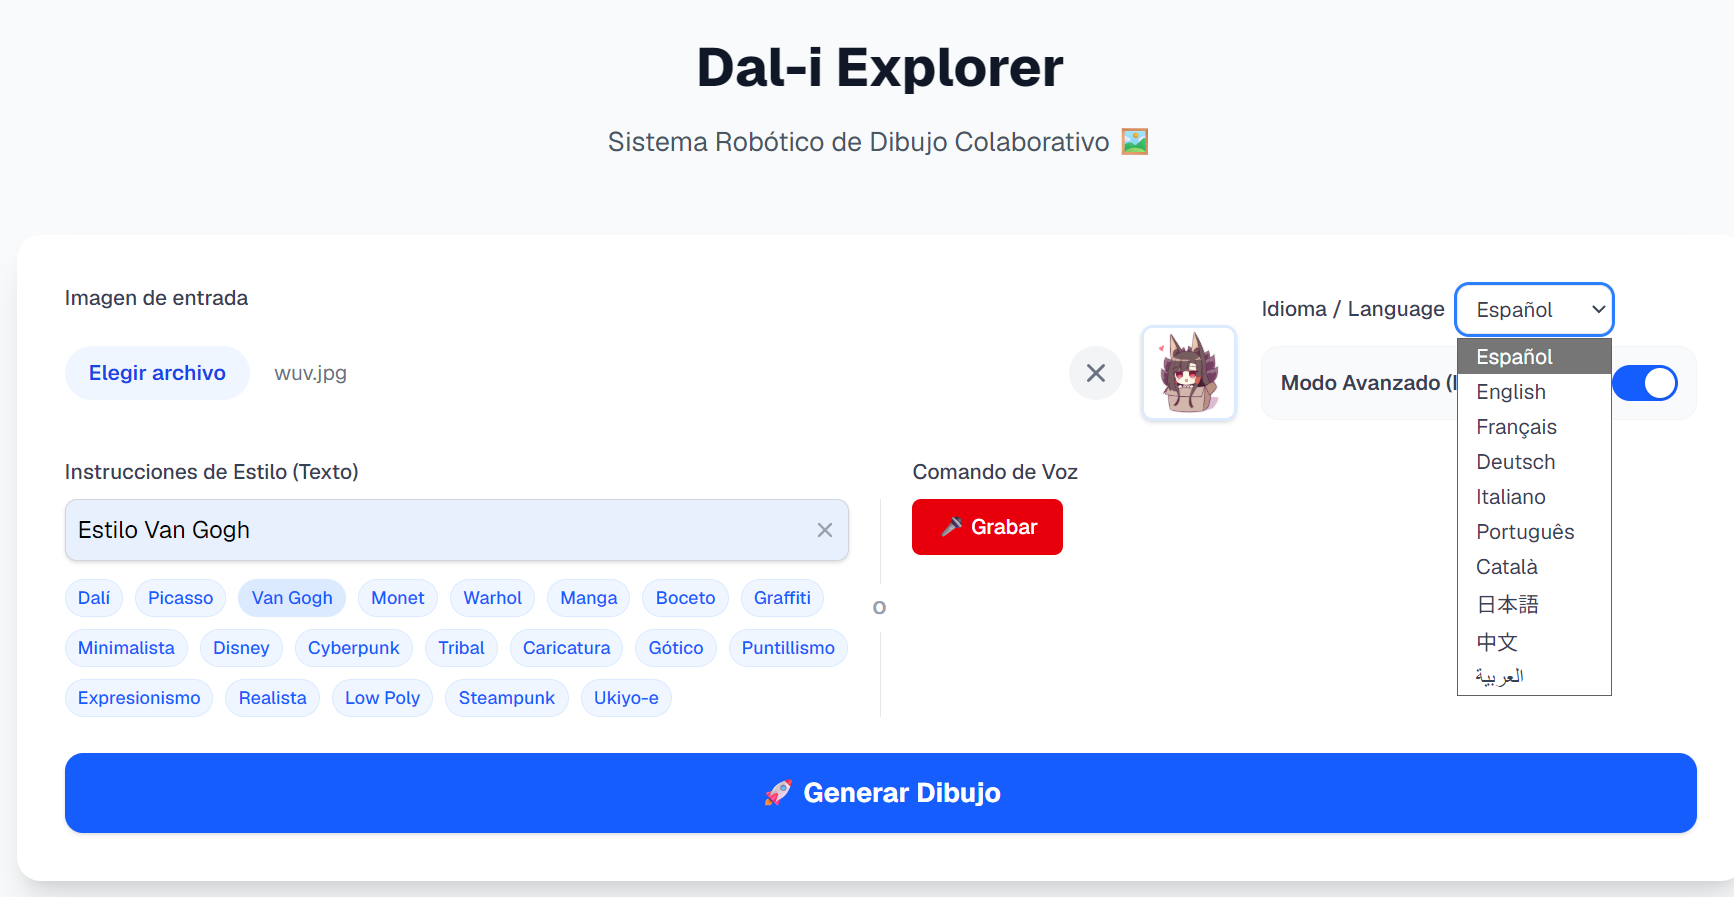
\includegraphics[width=\textwidth]{images/app_screenshot.png}
    %imgplaceholder[6.8cm]{images/app\_screenshot.png}
  \end{center}
\end{frame}


% ── Diapositiva 3: Tecnologies ───────────────────────────────
\begin{frame}{Tecnologies}
  \begin{columns}[T]

    \begin{column}{0.48\textwidth}
      \textbf{\color{dalblue}\faCloud\; Cloud (GCP)}
      \smallskip
      \begin{itemize}\small
        \item \alert{Cloud Run} — backend de visió (FastAPI)
        \item \alert{Cloud Functions ×3} — historial, upload,\\
              parla i traducció
        \item \alert{Vertex AI · Gemini 2.5 Flash} — estil visual
        \item Cloud Speech-to-Text · TTS · Translation
        \item Firestore · Cloud Storage
        \item Firebase Anonymous Auth
      \end{itemize}
    \end{column}

    \begin{column}{0.48\textwidth}
      \textbf{\faCog\; No-Cloud}
      \smallskip
      \begin{itemize}\small
        \item \alert{OpenCV} — Canny edge detection
        \item \alert{TSP} (Greedy NN + 2-opt)\\
              — optimització de trajectòries
        \item Next.js · React · TypeScript\\
              — frontend estàtic
        \item FastAPI · NumPy · Pillow
      \end{itemize}

      \medskip
      \begin{center}
        {\fontsize{52}{52}\selectfont\color{dalblue}\faCloud}\\[0.15cm]
        {\small\textbf{\color{dalblue}Google Cloud Platform}}
      \end{center}
    \end{column}

  \end{columns}
\end{frame}


% ── Diapositiva 4: Arquitectura ──────────────────────────────
\begin{frame}{Arquitectura}
  \begin{center}
  \begin{tikzpicture}[
      node distance=0.55cm and 0.7cm,
      box/.style={draw, rounded corners=4pt, minimum width=2.6cm,
                  minimum height=0.8cm, align=center, font=\small,
                  fill=dalblue!8, draw=dalblue!40},
      storage/.style={box, fill=gray!10, draw=gray!40},
      arr/.style={-{Stealth[length=5pt]}, thick, color=dalblue!70},
      lbl/.style={font=\scriptsize\color{gray}, midway}
    ]

    % ── Row 1: main pipeline ──────────────────────────────
    \node[box] (fe)  {\faDesktop\\[2pt]Frontend\\{\scriptsize Next.js · React}};
    \node[box] (cf)  [right=1.8cm of fe]
                     {\faCloud\\[2pt]Cloud Functions\\{\scriptsize history · upload · speech}};
    \node[box] (cr)  [right=1.8cm of cf]
                     {\faCog\\[2pt]Cloud Run\\{\scriptsize FastAPI · Vision}};

    % ── Row 2: data stores (below Cloud Run) ─────────────
    \node[storage] (fs) [below=0.7cm of cr]
                     {\faDatabase\\[2pt]Firestore + GCS};

    % ── Row 3: AI (below Cloud Functions) ────────────────
    \node[storage] (ai) [below=0.7cm of cf]
                     {\faBrain\\[2pt]Vertex AI · Gemini\\{\scriptsize Speech · TTS · Translate}};

    % ── Arrows ────────────────────────────────────────────
    \draw[arr] (fe)  -- node[lbl, above]{REST} (cf);
    \draw[arr] (cf)  -- node[lbl, above]{REST} (cr);
    \draw[arr] (cr)  -- (fs);
    \draw[arr] (cf)  -- (ai);

    % Firebase Auth annotation
    \node[font=\scriptsize\color{gray}, above=0.15cm of fe]
      {\faLock\; Firebase Anonymous Auth};

  \end{tikzpicture}
  \end{center}
\end{frame}


% ── Diapositiva 5: Resultats ─────────────────────────────────
\begin{frame}{Resultats}
  \vspace{0.3cm}
  \begin{columns}[c, onlytextwidth]
    \begin{column}{0.47\textwidth}
      \raggedleft
      \includegraphics[width=\linewidth, height=3.4cm, keepaspectratio]%
        {images/akagi pre.png}\\[0.1cm]
      \includegraphics[width=\linewidth, height=3.4cm, keepaspectratio]%
        {images/koharu pre.jpg}
    \end{column}
    \hspace{0.02\textwidth}
    \begin{column}{0.47\textwidth}
      \raggedright
      \includegraphics[width=\linewidth, height=3.4cm, keepaspectratio]%
        {images/akagi.png}\\[0.1cm]
      \includegraphics[width=\linewidth, height=3.4cm, keepaspectratio]%
        {images/koharu.jpeg}
    \end{column}
  \end{columns}
\end{frame}


% ── Diapositiva 6: Aportació a la Societat ───────────────────
\begin{frame}{Aportació a la Societat}

  % ── Meitat superior: robot SCARA centrat ─────────────────
  \begin{center}
    \begin{tikzpicture}[
        scale=3.8,
        joint/.style={circle, fill=dalblue, draw=dalblue!60!black,
                      line width=0.7pt, minimum size=10pt, inner sep=0pt},
        link/.style={line width=6pt, line cap=round, color=dalblue!75}
      ]
      \fill[gray!55, rounded corners=1.5pt]
        (-0.28,-0.04) rectangle (0.28, 0.04);
      \fill[gray!35, rounded corners=1pt]
        (-0.46,-0.13) rectangle (0.46,-0.04);
      \draw[line width=4.5pt, color=gray!55, line cap=butt]
        (0, 0.04) -- (0, 0.42);
      \node[joint] (J1) at (0, 0.42) {};
      \draw[link] (J1.east) -- (0.82, 0.42);
      \node[joint] (J2) at (0.82, 0.42) {};
      \draw[link, color=dalblue!55] (J2) -- (1.38, 0.02);
      \node[joint, minimum size=8pt, fill=dalblue!55] (J3) at (1.38,0.02) {};
      \draw[line width=4pt, color=gray!60, line cap=butt]
        (1.38, 0.02) -- (1.38,-0.18);
      \draw[line width=2pt, color=black!45]
        (1.38,-0.18) -- (1.38,-0.28);
      \fill[white]   (0.05,-0.36) rectangle (2.15,-0.32);
      \draw[gray!30, line width=0.5pt]
        (0.05,-0.36) rectangle (2.15,-0.32);
      \draw[dalblue!65, line width=1.6pt]
        (0.30,-0.34)
          .. controls (0.60,-0.29) and (0.85,-0.39) ..
        (1.10,-0.34)
          .. controls (1.30,-0.29) and (1.55,-0.37) ..
        (1.80,-0.34);
    \end{tikzpicture}
  \end{center}

  \vspace{-0.1cm}

  % ── Meitat inferior: dues columnes de beneficis ───────────
  \begin{columns}[T]
    \begin{column}{0.50\textwidth}
      \begin{itemize}\footnotesize
        \item[\alert{\faPalette}] \textbf{Creació Artística Democratitzada}\\
              \scriptsize Sense habilitats prèvies ni eines físiques
        \item[\alert{\faGlobeEurope}] \textbf{Accés Multilingüe}\\
              \scriptsize 10 idiomes, traducció automàtica en temps real
        \item[\alert{\faRobot}] \textbf{Pont Educatiu}\\
              \scriptsize IA generativa + robòtica + multimèdia
      \end{itemize}
    \end{column}
    \begin{column}{0.48\textwidth}
      \begin{itemize}\footnotesize
        \item[\alert{\faUniversalAccess}] \textbf{Potencial Terapèutic}\\
              \scriptsize Eina creativa accessible per a tothom
        \item[\alert{\faCloud}] \textbf{Arquitectura Serverless}\\
              \scriptsize Escalable i de baix cost
      \end{itemize}
    \end{column}
  \end{columns}

\end{frame}


\end{document}
